\documentclass[UTF8]{ctexart}
\usepackage{amsmath}
\usepackage{forest}
\usepackage{algorithm}
\usepackage{algorithmic}
\usepackage{tabularx}
\usepackage{booktabs}
\title{\vspace{-4cm}2023代组第四次作业}
\author{2000013058 杨仕博}
\date{\today}
\begin{document}
\maketitle

\subsection*{13}

下面每一题我们设给出的集合为W

(1)

若$A, B\in W$,则$(A-B)^T = A^T - B^T = A - B\Rightarrow A-B\in W$
,因而W是$M_n(R)$的子群。

(2)

若$A, B\in W$,设$A = diag\{a_1, a_2, ..., a_n\}, B = \{b_1, b_2, ..., b_n\}$
,$A - B = diag\{a_1 - b_1, a_2 - b_2, ..., a_n - b_n\}\in W$,
因而W是$M_n(R)$的子群。

(3)

由于全零矩阵$A$和只有左上角为1,其余位置为0的矩阵$B$都在$W$中,
但是$|A-B|<0\notin W$,因而W不是子群。

(4)

若$A,B\in W$是上三角矩阵,$A-B$也是上三角矩阵。因而$A - B\in W$。
所以W是$M_n(R)$的子群。

\subsection*{15}

(1)

考察$G = \{1\}, <G, \times, ^{-1}, 1>$构成了一个只有1个
元素的群,因而它只有1个子群。

(2)

考察$G = \{1, -1\}, <G, \times, ^{-1}, 1>$构成了一个只有2个
元素的群。由于$-1\times -1 = 1$,因而$<\{-1\}, \times, ^{-1}, 1>$
不构成群。同时,$<\{1\}, \times, ^{-1}, 1>, <\{1, -1\}, \times, ^{-1}, 1>$均
为群,因而$<G, \times, ^{-1}, 1>$是一个只有两个子群的群。

(3)

考察$G = \{1, -1, i, -i\}, <G, \times, ^{-1}, 1>$构成了
只有4个元素的群。由于在子群$W$中,$1\in W, i\in W\Leftrightarrow -i\in W \Rightarrow -1\in W$,
因而它的子群只有$<\{1\}, \times, ^{-1}, 1>, <\{1, -1\}, \times, ^{-1}, 1>, 
<G, \times, ^{-1}, 1>$三个。

\subsection*{16}

(1)

若$H_1H_2\leq G$,则

\[
\begin{aligned}
    &\forall h_1\in H_1, h_2\in H2, h_1^{-1}h_2^{-1}\in H_1H_2\\
    \Rightarrow &\forall h_1\in H_1, h_2\in H2, (h_2h_1)^{-1}\in H_1H_2\\
    \Rightarrow &\forall h_1\in H_1, h_2\in H2, ((h_2h_1)^{-1})^{-1}\in H_1H_2\\
    \Rightarrow &\forall h_1\in H_1, h_2\in H2, h_2h_1\in H_1H_2\\
    \Rightarrow & H_2H_1\subseteq H_1H_2
\end{aligned}
\]

\[
\begin{aligned}
    &\forall h_1\in H_1, h_2\in H2, (h_1h_2)^{-1}\in H_1H_2\\
    \Rightarrow &\forall h_1\in H_1, h_2\in H2, \exists g_1\in H_1, g_2\in H_2, s.t.\ (h_1h_2)^{-1} = g_1g_2\\
    \Rightarrow &\forall h_1\in H_1, h_2\in H2, \exists g_1\in H_1, g_2\in H_2, s.t.\ h_1h_2 = g_2^{-1}g_1^{-1}\in H_2H_1\\
    \Rightarrow &H_1H_2\subseteq H_2H_1
\end{aligned}
\]

故$H_1H_2 = H_2H_1$

(2)

若$H_1H_2 = H_2H_1$,

$\forall h_1, g_1\in H_1, h_2, g_2\in H_2$,

$h_1h_2(g_1g_2)^{-1} = h_1(h_2g_2^{-1})g_1^{-1}$,

$h_2g_2^{-1}\in H_2$,记$c_2 = h_2g_2^{-1}\in H_2$,则

$h_1(h_2g_2^{-1})g_1^{-1} = h_1c_2g_1^{-1}$

由$H_1H_2 = H_2H_1$,有$\exists b_1\in H_1, b_2\in H_2, s.t.\ h_1c_2g_1^{-1} = h_1b_1b_2$,

由$h_1b_1\in H_1$,有$h_1b_1b_2\in H_1H_2$,即

$h_1h_2(g_1g_2)^{-1}\in H_1H_2$,故$H_1H_2\leq G$

\subsection*{19}

(1)

模15的既约剩余系是$P = \{1, 2, 4, 7, 8, 11, 13, 14\}$,
$<a>$的生成元为$\{a^{i} | i\in P\}$中的元素。

(2)

由于对15的每个正因子d, 在G中有且仅有一个d阶子群,并且G中的每个
子群的阶均为15的因子,且$|<a^d>| = \frac{15}{(15, d)}$

因而$G$的全部子群为$<a>, <a^3>, <a^5>, \{e\}$

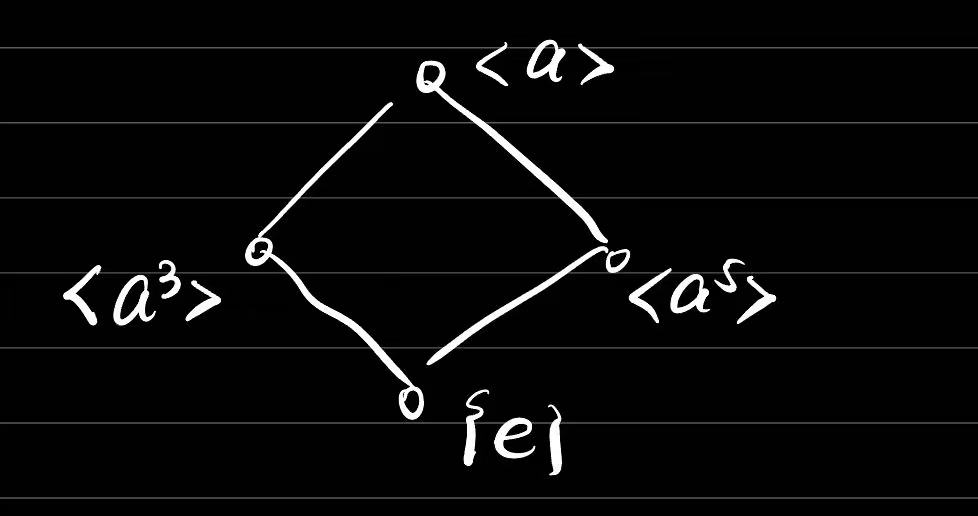
\includegraphics[width=.8\textwidth]{../pics/4.jpeg}

\subsection*{20}

首先,$e\in <a>, e\in B$

其次,若$\exists c\neq e\in <a>\bigcap <b>$,则可设
$c = a^i = b^j, i(\mod p)\neq 0$,于是$\exists r\in N, s.t.\ ir(\mod p) = 1$,
$a = a^{ir} = b^{jr}\in <b>$,矛盾!

因而,$<a>\bigcap <b> = \{e\}$

\end{document}